% Created 2021-09-09 jue 15:46
% Intended LaTeX compiler: pdflatex
\documentclass[11pt]{article}
\usepackage[utf8]{inputenc}
\usepackage[T1]{fontenc}
\usepackage{graphicx}
\usepackage{grffile}
\usepackage{longtable}
\usepackage{wrapfig}
\usepackage{rotating}
\usepackage[normalem]{ulem}
\usepackage{amsmath}
\usepackage{textcomp}
\usepackage{amssymb}
\usepackage{capt-of}
\usepackage{hyperref}
\usepackage[spanish]{babel}
\usepackage{fontspec}
\usepackage{float}
\usepackage{pdfpages}
\usepackage{fancyhdr}
\setmainfont{Noto Sans}
\setmainfont{Noto Sans}
\pagestyle{fancy}
\fancyhf{}
\rhead{
\includegraphics[width=0.05\textwidth]{assets/build/logo_nuevo_header}}
\lhead{Becos}
\rfoot{Página \thepage}
\author{Jonatan Ahumada \& Jorge Garzón}
\date{\today}
\title{Becos}
\hypersetup{
 pdfauthor={Jonatan Ahumada \& Jorge Garzón},
 pdftitle={Becos},
 pdfkeywords={},
 pdfsubject={},
 pdfcreator={Emacs 27.2 (Org mode 9.4.4)}, 
 pdflang={Spanish}}
\begin{document}



\begin{titlepage}
   \begin{center}
       \vspace*{1cm}

       \textbf{Plan de Negocios}

       
        
        
\includegraphics[width=0.8\textwidth]{assets/build/logotipo_nuevo}          
       \vspace{1.5cm}

       \textbf{Jonatan Ahumada \\
              Jorge Garzón}

       \vfill
           
               
       \vspace{0.8cm}
     

            
       Fundación Universitaria Konrad Lorenz\\
       Administración de Procesos de Negocio\\
       Bogotá, Colombia\\
 
            
   \end{center}
\end{titlepage}
\tableofcontents
\section{Análisis del entorno}
\label{sec:org445c03c}
\subsection{PESTEL}
\label{sec:org37f1fc5}
\subsubsection{Político}
\label{sec:org379aa8c}
\begin{enumerate}
\item Amenaza de variante delta y mu
\label{sec:orgd299be5}

Con la aparición de nuevas variantes, la comunidad internacional está
considerando volver a implementar medidas de aislamiento.

Esto es una \textbf{amenaza} porque la infraestructura física requiere un
plantel de trabajadores para sus procesos de confección, que está
ligado a la mano de obra de las trabajadoras. Habra más costos para
garantizar la salubridad y hay límites de espacio que se deben
respetar, lo que disminuye capacidad de producción

\item Cese de presencialidad en los colegios
\label{sec:orgb222d56}

Si se prolonga el aislamiento social, por un posible cuarto pico, la
proyección de ventas se desploma, puesto que prinipalmente recae en
escuelas de futbol y colegios de Bogotá, que participan en torneos
locales.

Esto es una \textbf{amenaza} porque no habrá demanda de uniformes por
parte de ese segmento.


\item Déficit fiscal y tributación de la reforma 2.0:
\label{sec:orga5490bc}

En la nueva reforma fiscal la tarifa de renta subirá del 30 al 35\%
para hacerle frente al déficit fiscal que enfrenta el país.

Esto es una \textbf{amenaza} porque los márgenes de rentabilidad será más
estrecho.  Más aun, teniendo en cuenta el costo competitivo que el
plan de negocios plantea para sus productos.
\end{enumerate}

\subsubsection{Económico}
\label{sec:org343ccb7}
\begin{enumerate}
\item Alsa del dólar
\label{sec:org32cb05a}
  
La amenaza de la variante delta hace que la Fed aumente las tasas de
interés del dolar, lo que desvaloriza el peso colombiano frente a la
divisa.

Esto es una \textbf{amenaza} porque puede disuadir la inversión extranjera
en el sector textil. Esto puede reducir los márgenes de
rentabilidad de la confección, manufactura y distribución
de producto textil.
\end{enumerate}


\subsubsection{Social}
\label{sec:org12d2e36}
\begin{enumerate}
\item Protagonismo del sector textil colombiano a nivel internacional
\label{sec:orgbda6197}

El sector textil y la moda registra el 37\% de las empresas registrados en CCB.
Según Colombia Productiva, el sector textil y de confección es el primer
generador de mano de obra en la industria nacional. Además, Colombia es el
primer exportador de tejido plano en Suramérica.

Esto es una \textbf{oportunidad} porque el reconocimiento externo de la moda colombiana
podría formar sinergía con una de las propuestas diferenciadoras de Becos:
ayudar a madres cabezas de hogar de sectores vulnerables a la vez que se
contribuye al medio ambiente, dado que estos son temas coyunturales.

\item Necesidad de impulsar la reactivación económica
\label{sec:orge503cd2}

El Gobierno Duque enfatiza que el pais muestra ritmo de crecimiento
elevado (1,1\%) el primer trimestre del año, en comparación con paises
como Chile o México. El gobierno pronostica un desarrollo favorable
durante el resto del año.

Esto es una \textbf{oportunidad} porque parece improbable que el gobierno
actual paralice la reactivación ecónomica, más aún si se se han hecho
esfuerzos presupuestales para iniciar le proceso de vacunación.
\end{enumerate}

\subsubsection{Tecnológico}
\label{sec:org553a00d}
\begin{enumerate}
\item Costos en servicios web
  \label{sec:org7f15774}
  
Los servicios de Cloud Computing de Amazon se cotizan en dólares.
Este servicio es parte crucial de la infraestructura tecnolgócia

Esto es una \textbf{amenaza} porque aumenta los costos en infraestructua
\item Escasez de profesionales TI
\label{sec:org933a81f}

Esto es una \textbf{amenaza} heredada del mercado de talento humano
colombiano, ya que a día de hoy existe una demanda superior a la
oferta en cuanto a profesionales TI.
\end{enumerate}

\subsubsection{Ambiental}
\label{sec:org9187abc}
\begin{enumerate}
\item Aceptación cultural del reciclaje
  \label{sec:orgebeefdc}
  
El mundo está entrando en periodo de conciencia ambiental. En
Colombia, sectores como el de los hidrocarburos están iniciado una
transformación hacia energías más limpias.

Esto es una \textbf{oportunidad}, puesto que hay una tendencia cultural
por participar en la genereción de un mundo ecosostenible, lo
que hace que la propuesta de Becos altamente atractiva en el pais
y el mundo por igual.
\end{enumerate}
\subsubsection{Legal}
\label{sec:org109c92b}
\begin{enumerate}
\item Beneficios de una Sociedad por acciones simplificada
\label{sec:org5580340}

En Colombia, estar constituido de esta manera representa una
\textbf{oportunidad}, dadas las exenciones tributarias que conlleva.

\item Beneficios ambientales
\label{sec:orgf16b6a1}

Se considera una \textbf{oportunidad} ya que la propuesta de Becos también
pretende ser referente a nivel de leyes.
\end{enumerate}
\subsection{5 Fuerzas}
\label{sec:org7915404}
\begin{figure}[H]
\centering
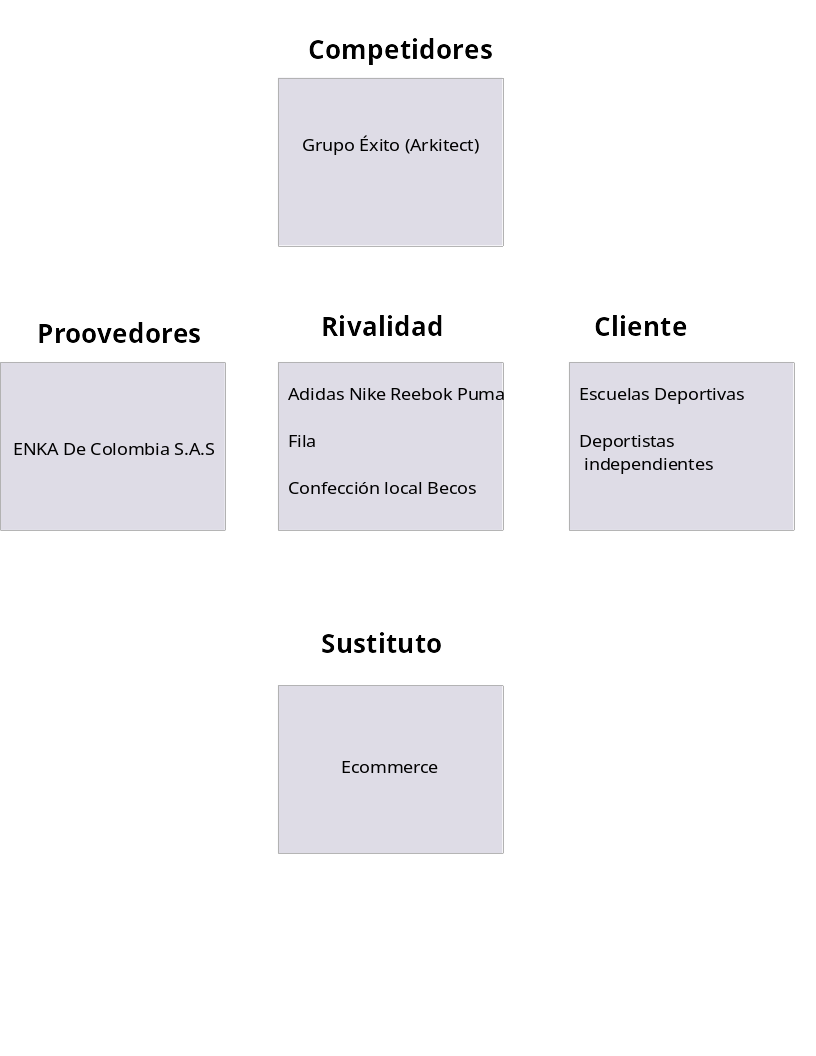
\includegraphics[width=.9\linewidth]{./assets/build/5_fuerzas.png}
\caption{\label{fig:orge49e3f4}5 fuerzas de Porter}
\end{figure}

\section{BMM}
\label{sec:orgbe8d077}
\subsection{Misión y vision}
\label{sec:org0a61fe2}
\subsubsection{Misión}
\label{sec:org5715524}
Ser referente nacional e internacional con respecto
a procesos ecologicamente sostenibles en el sector
textil. Unir el diseño de la moda colombiana
con la sostenibilidad y la conciencia social.

\subsubsection{Visión}
\label{sec:org57cb682}

Para el año 2025, BECOS tendrá toda todo un catálogo de ropa deportiva
fabricada con elementos 85\% reciclados. Tendrá lineas de ropa deportiva para
todos los deportes que demanden indumentaria deportiva, desde los más
practicados por los colombianos: fútbol, basquetból, ciclismo, tenis, entre
otros, hasta los de díficil adquisición: danza, ballet, patinaje,
deportes urbanos etc.

\subsection{Assesment}
\label{sec:org30cf688}
\begin{enumerate}
\item Influencias
\label{sec:orge474aff}

\begin{enumerate}
\item Externas

\begin{itemize}
\item Gobierno Colombiano
\item Mercado Internacional
\item Confeccionistas de Bogotá
\end{itemize}
\end{enumerate}


\begin{enumerate}
\item Internas

\begin{itemize}
\item Adecuación a protocolos de Bioseguridad
\item Implementación de hardware y software
\end{itemize}
\end{enumerate}

\item DOFA
\label{sec:orgfce53f4}
\begin{figure}[H]
\centering
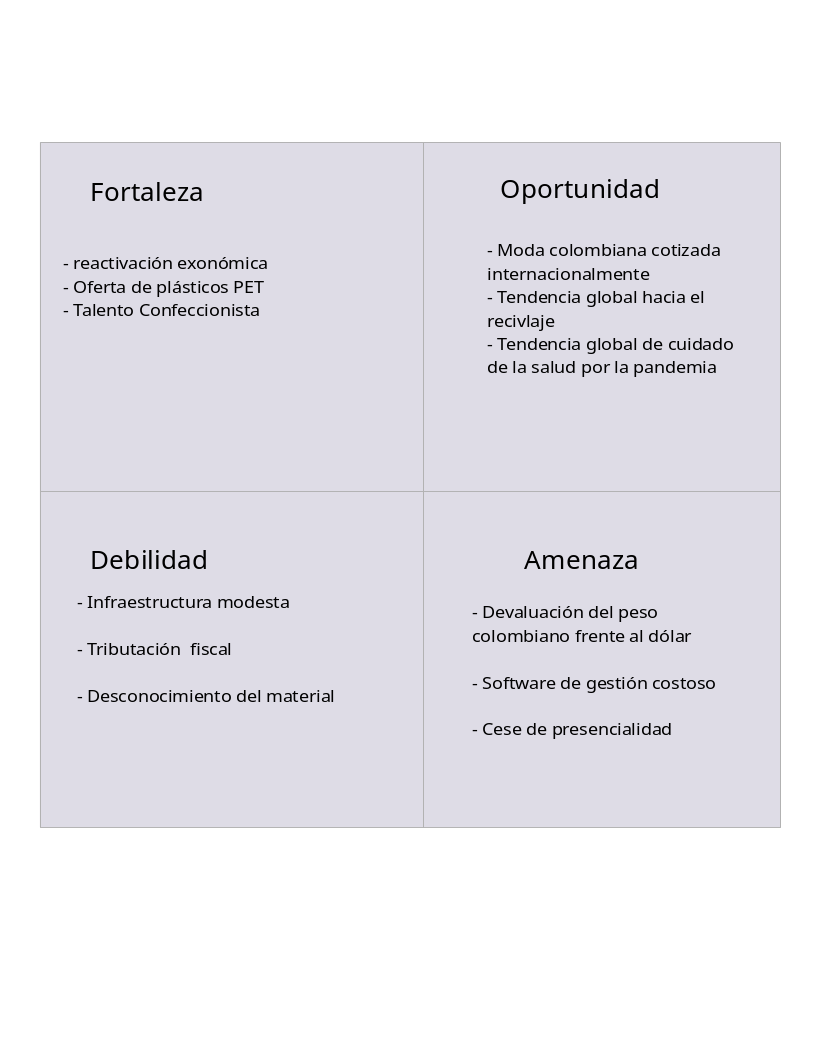
\includegraphics[width=.9\linewidth]{./assets/build/dofa.png}
\caption{\label{fig:org3d53f5c}DOFA para Assesment de Influencias}
\end{figure}
\end{enumerate}


\subsubsection{Medios}
\label{sec:orged4e532}

\begin{figure}[H]
\centering
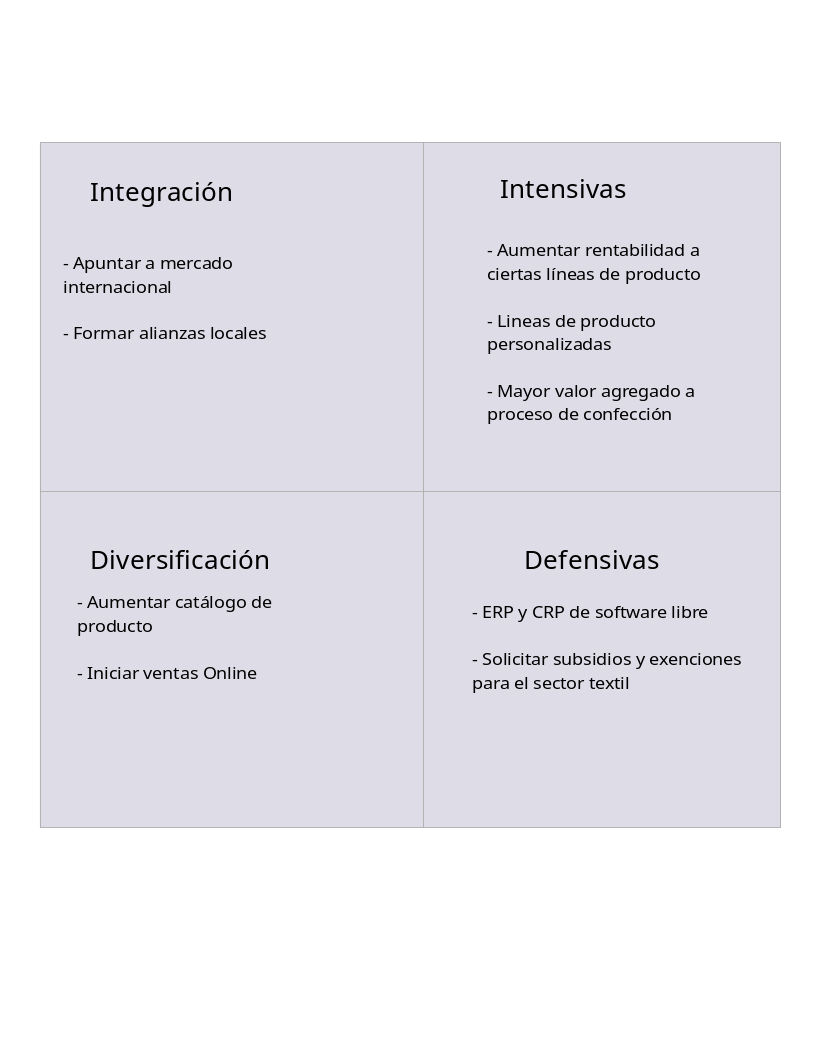
\includegraphics[width=.9\linewidth]{./assets/build/means.png}
\caption{\label{fig:orgc401d31}Estrategia}
\end{figure}

\subsubsection{Externas}
\label{sec:orgd3c9b75}

\subsection{Blue Ocean Strategy Canvas \& ERRC GRID}
\label{sec:org22b177e}
Ver figuras \ref{fig:blue_ocean}, \ref{fig:ercc}

\begin{figure}[H]
\centering
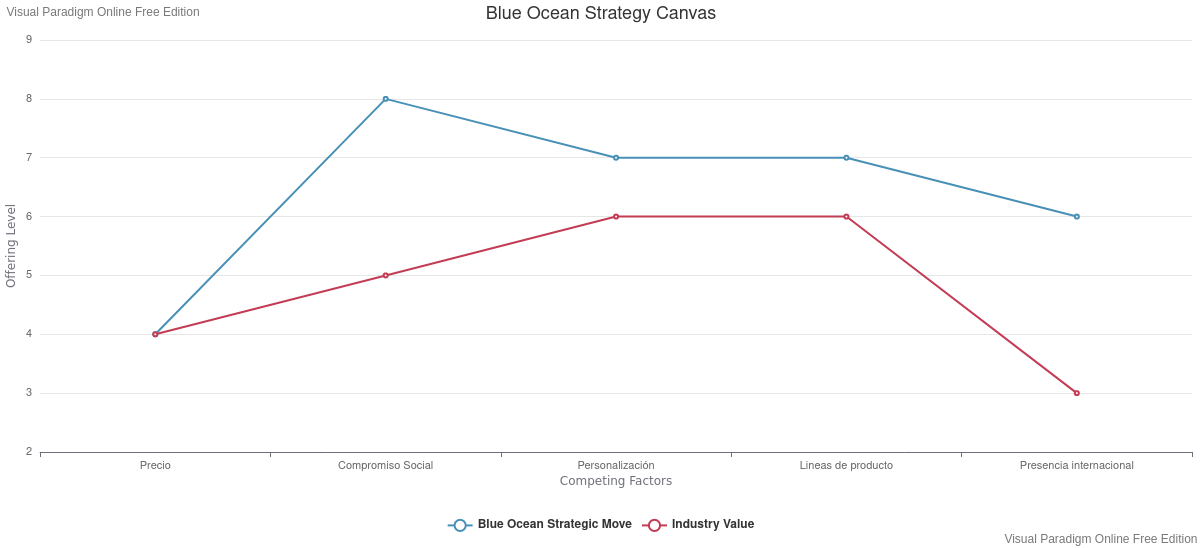
\includegraphics[width=.9\linewidth]{./assets/build/blue_ocean_canvas.png}
\caption{\label{fig:blue_ocean}Blue Ocean Strategy Canvas}
\end{figure}
\begin{figure}[H]
\centering
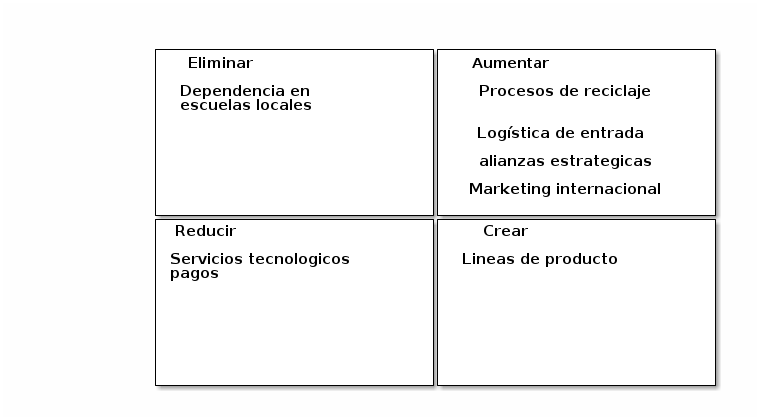
\includegraphics[width=.9\linewidth]{./assets/build/ercc.png}
\caption{\label{fig:ercc}ERRC}
\end{figure}
\subsection{Mapa de procesos, diccionario de procesos y organigrama}
\label{sec:org80ff363}

\begin{figure}[htbp]
\centering
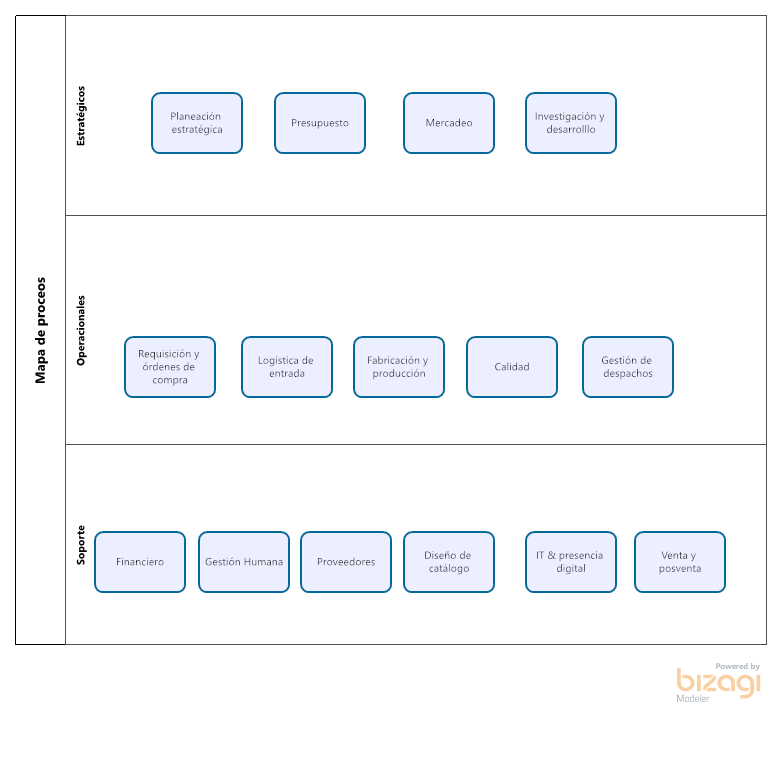
\includegraphics[width=.9\linewidth]{./assets/build/mapa_procesos.png}
\caption{\label{fig:mapa_procesos}Mapa de procesos}
\end{figure}

\begin{figure}[htbp]
\centering
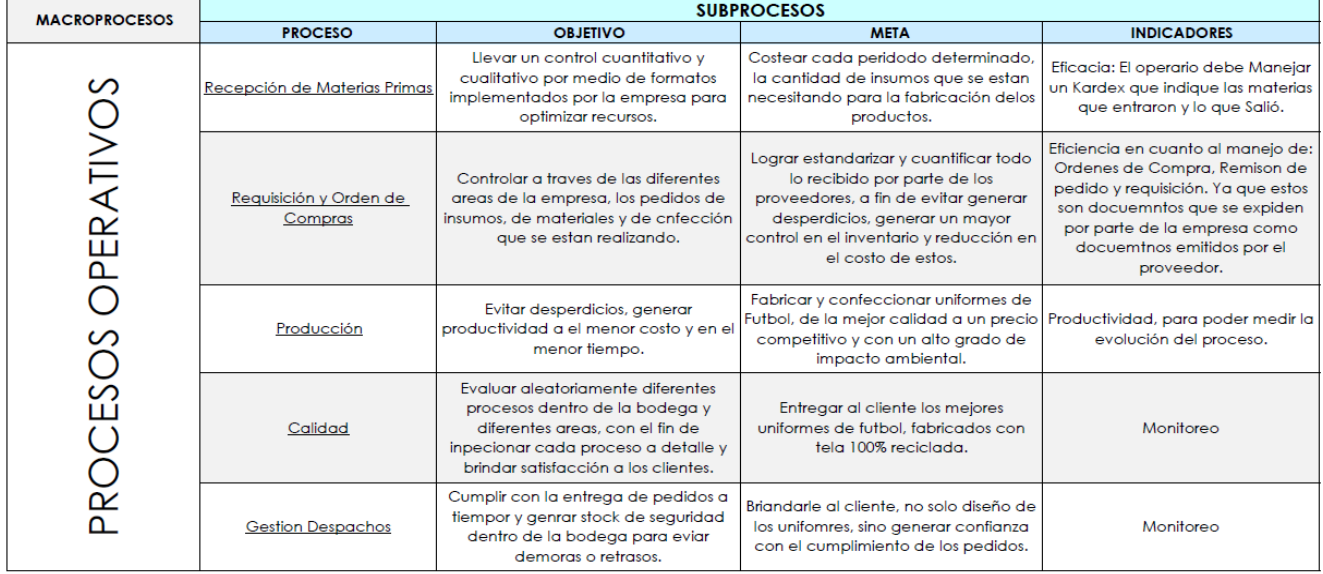
\includegraphics[width=.9\linewidth]{./assets/build/diccionario_procesos.png}
\caption{\label{fig:dic_procesos}Diccionario de Procesos}
\end{figure}

\begin{figure}[htbp]
\centering
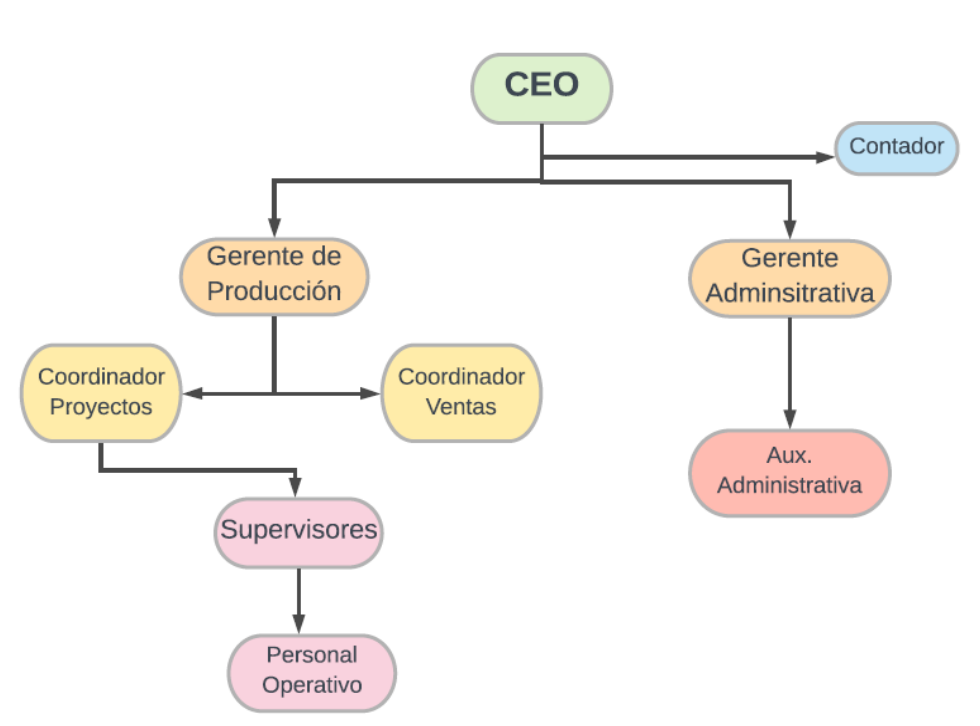
\includegraphics[width=.9\linewidth]{./assets/build/organigrama.png}
\caption{\label{fig:organigrama}Organigrama}
\end{figure}

Ver figuras \ref{fig:mapa_procesos}, \ref{fig:dic_procesos}, \ref{fig:organigrama}.

\subsection{Procesos estratégicos}

Ver figuras \ref{fig:planeacion}, \ref{fig:presupuesto}, \ref{fig:mercadeo}.
\begin{figure}[H]
\centering
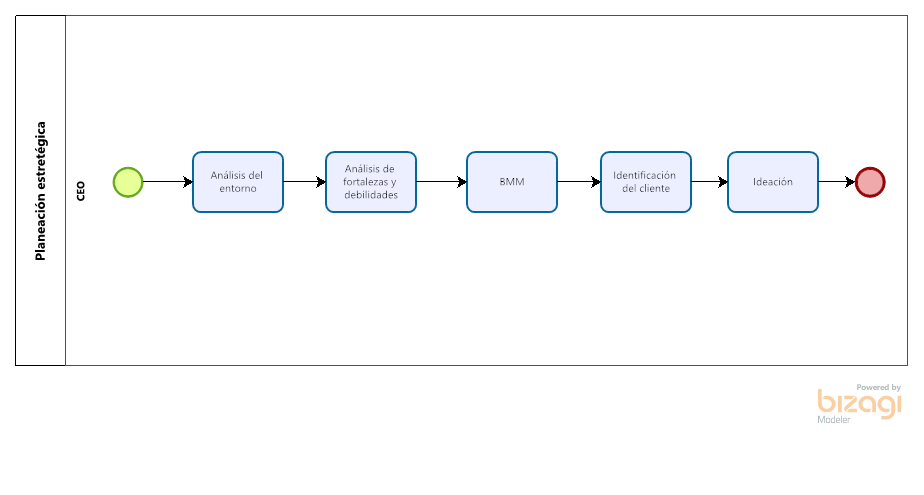
\includegraphics[width=.9\linewidth]{./assets/build/planeacion.png}
\caption{\label{fig:planeacion}Planeación estratégica}
\end{figure}

\begin{figure}[H]
\centering
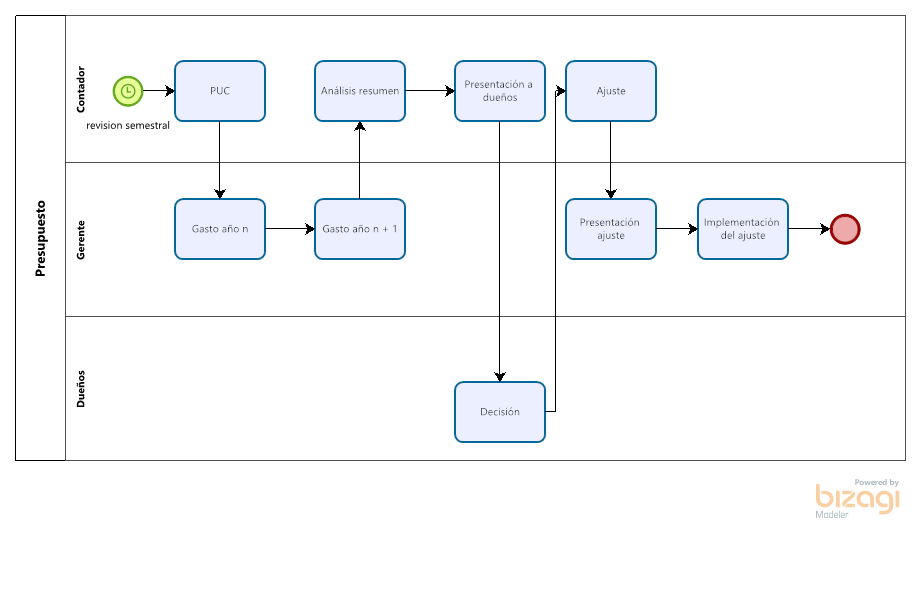
\includegraphics[width=.9\linewidth]{./assets/build/presupuesto.png}
\caption{\label{fig:presupuesto}Presupuesto}
\end{figure}

\begin{figure}[H]
\centering
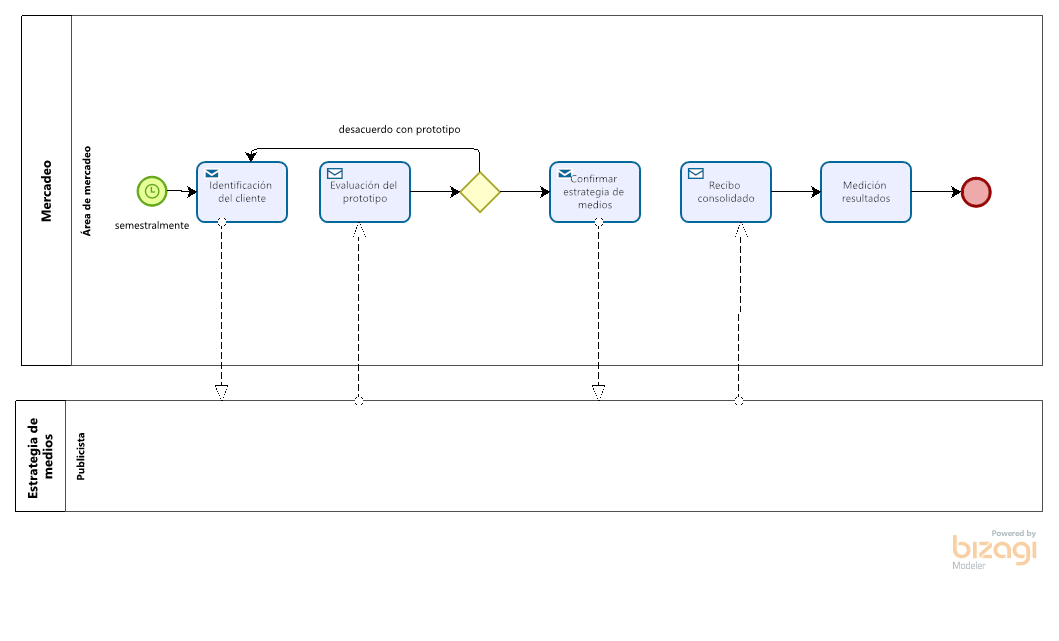
\includegraphics[width=.9\linewidth]{./assets/build/mercadeo.png}
\caption{\label{fig:mercadeo} Mercadeo}
\end{figure}

\begin{figure}[H]
\centering
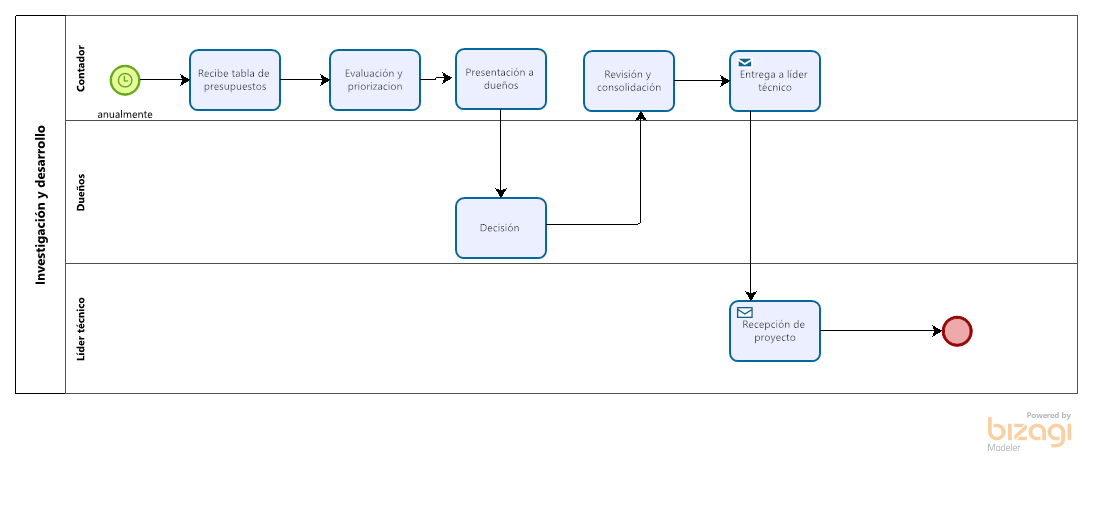
\includegraphics[width=.9\linewidth]{./assets/build/investigacion.png}
\caption{\label{fig:investigacion} Investigación y desarrollo}
\end{figure}

\subsection{Procesos operativos}
\begin{figure}[H]
\centering
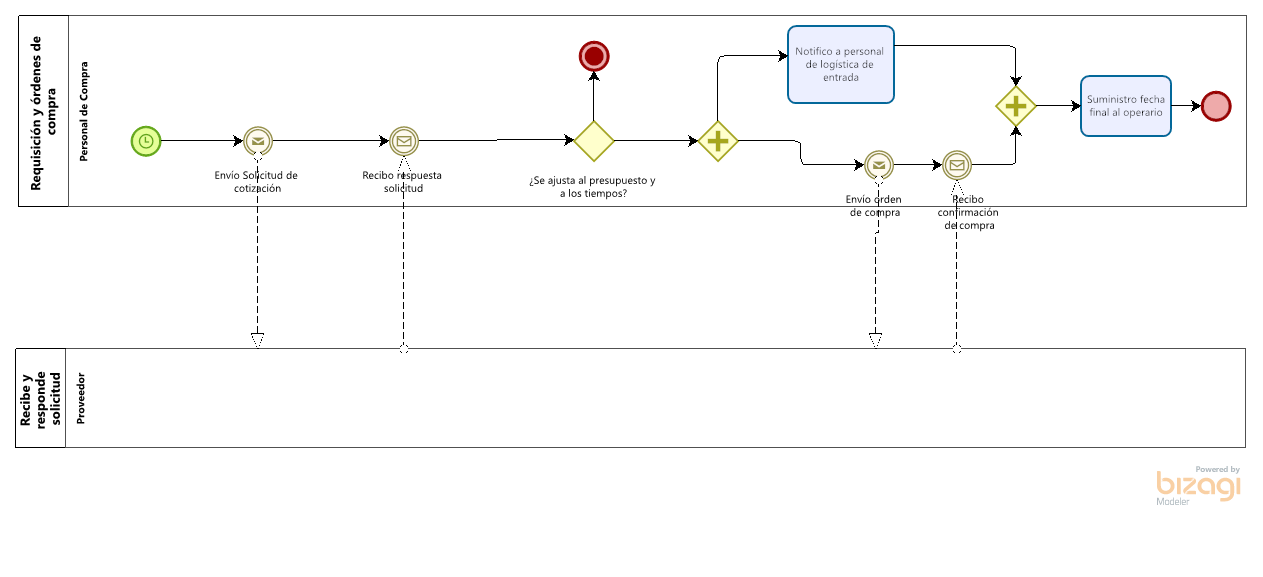
\includegraphics[width=.9\linewidth]{./assets/build/requisicion_compra.png}
\caption{\label{fig:req_compra}Requisición y compra}
\end{figure}

\begin{figure}[H]
\centering
\includegraphics[width=.9\linewidth]{./assets/build/logística_entrada.png}
\caption{\label{fig:log_entrada}Logística de entrada}
\end{figure}

\begin{figure}[H]
\centering
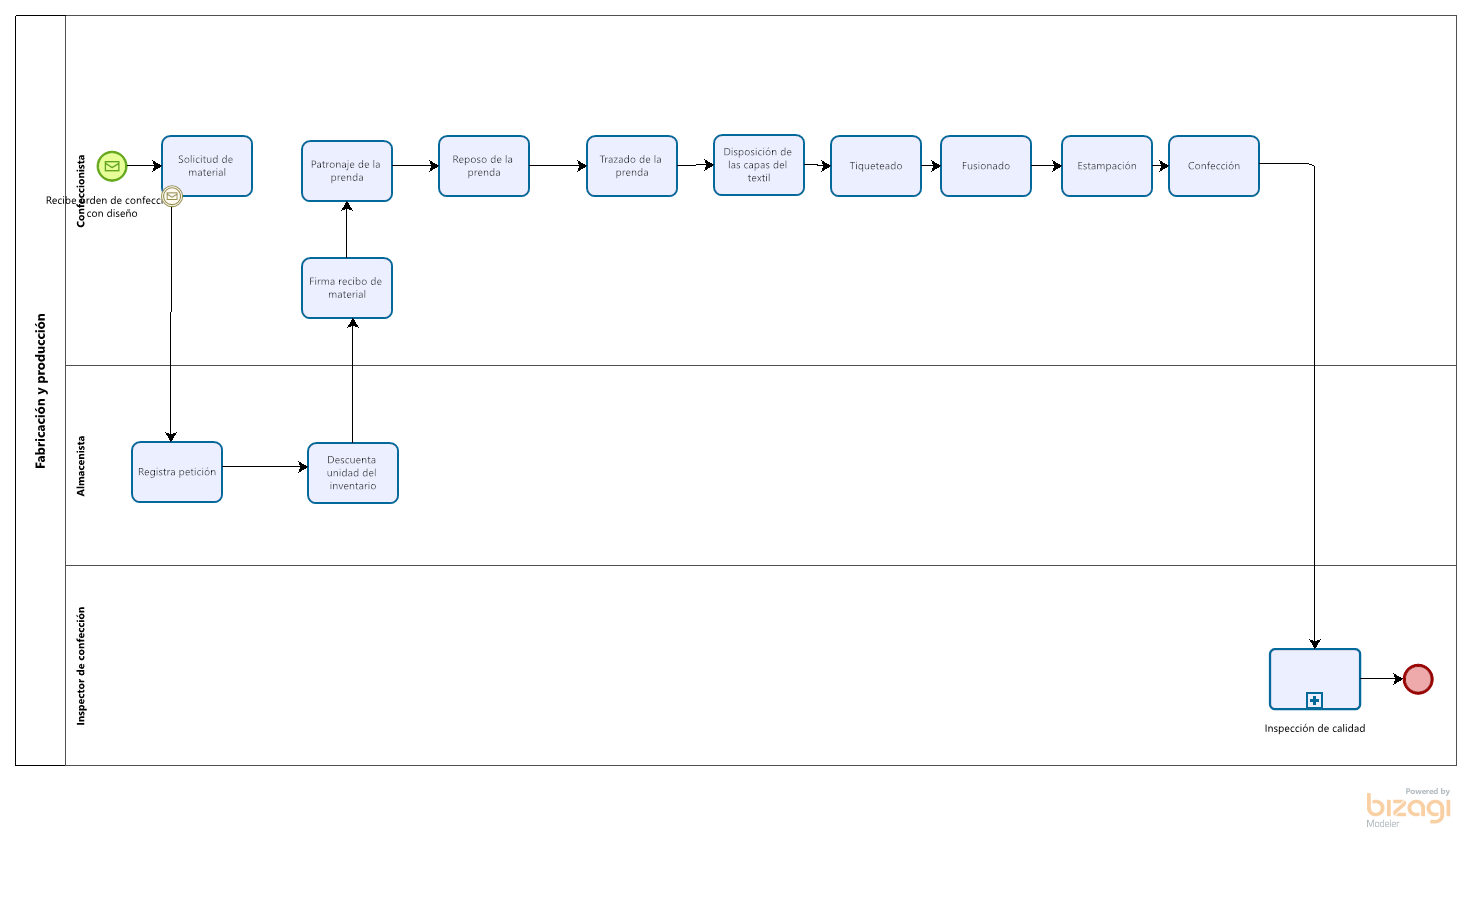
\includegraphics[width=.9\linewidth]{./assets/build/fabricacion_produccion.png}
\caption{\label{fig:fab_prod}Fabricación y producción}
\end{figure}

\begin{figure}[H]
\centering
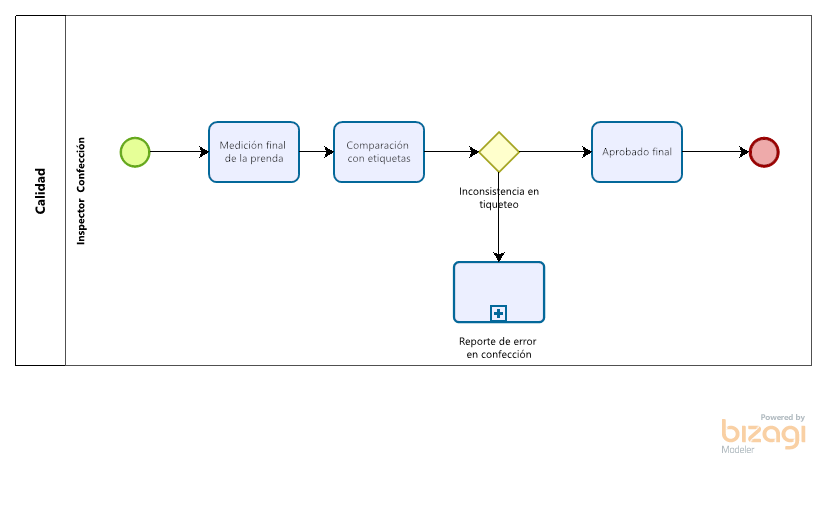
\includegraphics[width=.9\linewidth]{./assets/build/calidad.png}
\caption{\label{fig:calidad} Calidad}
\end{figure}

\begin{figure}[H]
\centering
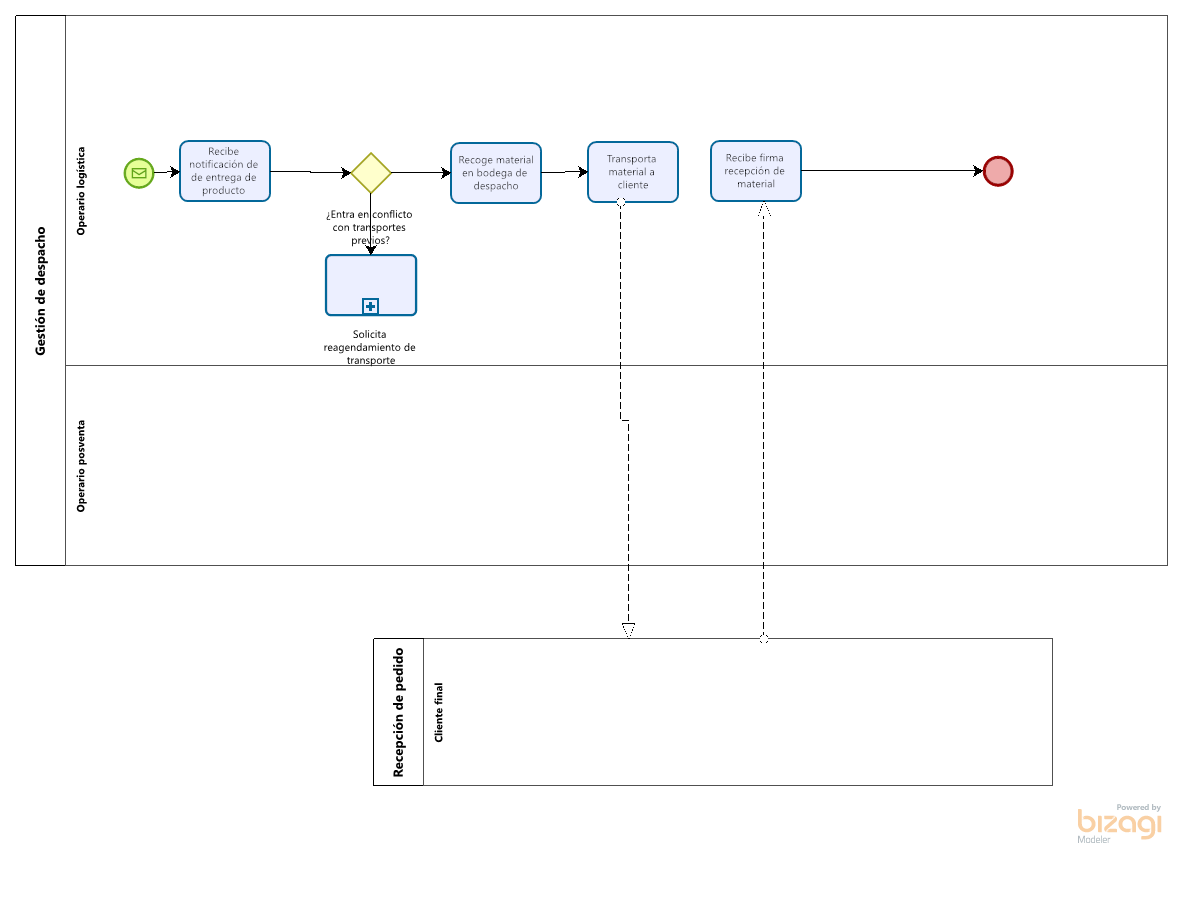
\includegraphics[width=.9\linewidth]{./assets/build/gestion_despacho.png}
\caption{\label{fig:gest_despacho}Gestión de despachos}
\end{figure}

\section{Buyer Persona}
\label{sec:org8fcde79}
\subsubsection{Definición del segmento de clientes}
\label{sec:org14c8273}
Los clientes potenciales de BECOS son principalmente
dos segmentos.

\begin{enumerate}
\item Padres de niños en escuelas de fútbol

El segmento principal de BECOS son
las escuelas de fútbol, puesto
que presentan la necesidad
de adquirir un uniforme.
Sin embargo, en este momento
este segmento está en amenaza,
por las restricciones en la
presencialidad de los colegios
y la prohibición de aglomeraciones.
Aunque el usuario final es un niño
o joven menor de 18, los clientes
son padres de un rango variable de
edad.
\end{enumerate}


\begin{enumerate}
\item Deportistas de equipos independientes 

En Bogotá se observa que las
canchas de los parques públicos se utilizan
para jugar extra-oficialmente. Es decir,
sin necesidad de estar inscritos en una
escuela. Por lo general, los usuarios
forman equipos regulares de amigos, o
conocidos del área que podrían estar
interesados en adquirir un uniforme,
para añadir un 'plus' a sus partidos
recreaionales.

\begin{enumerate}
\item Deportistas individuales

Junto a los deportistas que juegan en grupos
de amigos, se observa que hay también un
segmento considerable de personas que
realizan actividades deportivas de manera
individual y que pueden tener necesidad
de un producto confeccionado a la medida.
Por ejemplo, personas que trotan, que
entrenan con entrenador personal, que
realizan ejercicios de calistenia, etc.
\end{enumerate}
\end{enumerate}



\subsubsection{Entrevistas}
\label{sec:orgde70a25}
En total se hicieron 10 entrevistas. Aquí dejamos una
muestra a manera de ejemplo:

\begin{verse}
\vspace*{1em}
\vspace*{1em}
\vspace*{1em}
- ¿juegas en algún equipo de fútbol, tienen uniformes?\\
\hspace*{2em}Sí. Mi hijo. ( lo señala)\\
- ¿Tuviste alguna capacidad de decisión en cuanto al uniforme de tu equipo?\\
\hspace*{2em}No.\\
\vspace*{1em}
\vspace*{1em}
- ¿Quien te pareció que tuvo el factor decisivo en la decisión?\\
\vspace*{1em}
\hspace*{2em}La verdad no sé porque mi esposo es el que ha estado interactuando. Pero mi amgino que son los preofesores con algun proveedor no?. Y tuvieron que haber tenido en cuenta la disciplina\\
\vspace*{1em}
- ¿Estuviste de acuerdo con la decisición del uniforme?\\
\vspace*{1em}
\hspace*{2em}Sí. me parece que son los idóneos\\
\vspace*{1em}
- ¿Estás satisfecho con la calidad de tu uniforme, le cambiarías algo?\\
\vspace*{1em}
\hspace*{2em}No porque son uniformes bastante amplios, cómodos. No definen la\\
\hspace*{2em}figura de algun modo.\\
\vspace*{1em}
-¿Te orma bien tu uniforme?\\
\hspace*{2em}(El entendido es que no )\\
\vspace*{1em}
\vspace*{1em}
- ¿Te gusta estéticamente tu uniforme?\\
\vspace*{1em}
\hspace*{2em}Le cambiará el color porque ese tono de rojo no me\\
\hspace*{2em}llama mucho la atencion.\\
\hspace*{2em}Muy chillón.\\
\vspace*{1em}
\hspace*{2em}Me gusta más el azul de la chica aquella\\
\vspace*{1em}
Precio\\
\vspace*{1em}
- ¿Te parece justo el precio que pagaste por los uniformes que has comprado?\\
\vspace*{1em}
\hspace*{2em}En particular no lo he comprado porque mi hijo es nuevo. Esta es una clase de\\
\hspace*{2em}cortesía.\\
\vspace*{1em}
- ¿Te parece que un precio entre  45,000 y 48,000  es competitivo para un uniforme (camisa y pantaloneta) en Bogotá?\\
\vspace*{1em}
\hspace*{3em}La verdad me parece ecónomico (sonríe).\\
\vspace*{1em}
- ¿Pagarías más para tener más opciones de personalización en tu uniforme?\\
\vspace*{1em}
\hspace*{2em}Depronto no por el tema de personalizacion sino por ejemplo, la textura de la tela.\\
\vspace*{1em}
\hspace*{3em}Por ejemplo, los uniformes de Adidas que son telas especializadas\\
\hspace*{3em}para el sudor. Si me ofrecen telas así especializadas, si estaría\\
\hspace*{3em}dispuesta a pagar más.\\
\vspace*{1em}
\vspace*{1em}
\vspace*{1em}
\vspace*{1em}
factor diferenciador\\
\vspace*{1em}
- ¿Le prestas atención al material del uniforme, sabes de qué estan hechos los uniformes que has comprado anteriormente?\\
\vspace*{1em}
\hspace*{2em}Sí. Me parece realmente importante. Me parece uno de los temas más importantes.\\
\hspace*{2em}¿conoces de qué están hechos los uniformes de Adidas?\\
\hspace*{2em}Pues, que yo te diga especificamente no. Porque no tengo estudios sobre el tema.\\
\hspace*{2em}Pero cuando una va a una iende de adidas uno suelde explicarles a uno prque tiene este sistema.\\
\hspace*{2em}le explican a uno las especificaciones y cuales son los beneficios de pagar ese costo por el producto\\
\vspace*{1em}
\hspace*{2em}- ¿Conoces los beneficios del PET como tejido textil?\\
\hspace*{2em}No. Ni idea\\
- Ahora que los conoces:\\
- ¿Te importaría positivamente si los uniformes están hechos con un alto grado de plastico PET desechable para contruibir al planeta?\\
\vspace*{1em}
\hspace*{2em}Sí. Me llamaria la atencion porque contribuye al planeta pero siempre y cuando no genera ninguna enfermedad para el cuerpo de mi hijo. Alguna reaccion en la pioel  Me imagino que eso tiene un proceso ideoneo para asegurar su uso.\\
\vspace*{1em}
- ¿Te importaría negativamente si los uniformes están hechos con un alto grado de plástico PET desechable para contribuir al planeta?\\
\vspace*{1em}
\hspace*{2em}N.A\\
\vspace*{1em}
- ¿Conoces cómo confeccionaron los uniformes que has comprado anteriormente?\\
\hspace*{2em}No.\\
\vspace*{1em}
- ¿Te importaría positivamente si los uniformes están confeccionados por madres cabeza de hogar?\\
\vspace*{1em}
\hspace*{2em}Me parecería espectacular. Entre una persona del comun y una madre cabeza de hogar por su puesto que me de decantarpia por\\
\hspace*{2em}una madre cabeza de hogar.\\
\vspace*{1em}
- ¿Te interesaría poder diseñar uniformes?\\
\vspace*{1em}
- ¿Te interesarí ir a premisas (a la fabrica), para comprobar tonalidades de color y medidas de la prenda antes de producir el producto?\\
\hspace*{2em}No. Me hstaria que ellos que fueron los que estudiaron, los diseñen y me los muestren y yo lo escogeria.\\
\hspace*{2em}Pero participar con eldiseño como tal, no, porque no es algo sea de mi interes. Pero depronto sí estar pendiende que\\
\hspace*{2em}sea un diseño bonito\\
- ¿Has comprado algun uniforme que te ofrezca personalización anteriormente?\\
\vspace*{1em}
\hspace*{2em}No.Practicamente lo que el colegio ofrece, los colores ,los textiles. Uno está supeditado a lo que el colegio ofrece.\\
\vspace*{1em}
\hspace*{2em}¿Como madre te gustaria participar?\\
\vspace*{1em}
\hspace*{3em}Sí me gustaria porque particularmente los uniformes del colegio de mi hija a mí nunca me han gustado.Son chillones.\\
\hspace*{3em}Uy. Fuchsia con un azúl terrible.\\
\vspace*{1em}
- ¿Has comprado a algún confeccionista en Bogotá que te ofrezca validación de colores y medidas antes de comprar el uniforme?\\
\hspace*{2em}No.\\
\vspace*{1em}
diversificacion\\
- ¿Te interesaria cotizar uniformes por internet y luego validarlos en premisa?\\
\vspace*{1em}
\hspace*{2em}Sí. Me parece una buena metodología. Más ahora en esta epoca de pandemia. Si hay la oportunidad de verlos asú y no tener que ir a un lugar y exponerse muchísimo mejor.\\
\vspace*{1em}
- ¿Te interesaria tener otros productos de un material similiar y estética al de tu uniforme?\\
- ¿Puedes nombrar alguno que te interese (buzos, gorras, bolsos, etc, ropa casual)?\\
\vspace*{1em}
\hspace*{2em}Sí. Derponto para patinaje. Por lo general uno no ve uniformes así en esa disciplina. Mira que\\
\hspace*{2em}si tu vas a escuales de patinaje o cursos de patinaje, normalmente no piden uniforme.\\
\vspace*{1em}
\hspace*{2em}¿Tu hija o hijo a estado?\\
\hspace*{2em}Sí. Mi hijo y no le pidieron uniforme\\
\vspace*{1em}
\hspace*{2em}¿Y a tí como madre te gustaria darle el uniforme, para que se siente más cómodo practicando\ldots{}?\\
\vspace*{1em}
\hspace*{2em}Sí. Porque por ejemplo cuando empezó el curso rompió dos sudaderas. Eran sudaderas\\
\hspace*{2em}costosas. de marca. En cambio con un uniforme de esos pues si se rompe uno dice\\
\hspace*{2em}el costo no fue tan alto.\\
\vspace*{1em}
\hspace*{2em}Que sea un atuendo que se pueda poner para practicar ese deporte específicamente.\\
\vspace*{1em}
\hspace*{2em}Gracias\\
\end{verse}
\subsubsection{Encuesta}
\label{sec:orgf4cb41c}
Esta encuesta se circuló en redes sociales,|
pero no alcanzó un valor representativo.

\begin{verse}
Aspectos del producto\\
- ¿juegas en algún equipo de fútbol, tienen uniformes?\\
- ¿Tuviste alguna capacidad de decisión en cuanto al uniforme de tu equipo?\\
- ¿Quien te pareció que tuvo el factor decisivo en la decisión?\\
- ¿Estuviste de acuerdo con la decisición del uniforme?\\
- ¿Estás satisfecho con la calidad de tu uniforme?\\
- ¿Te orma bien tu uniforme?\\
- Si no, ¿qué le mejorarías?\\
- ¿Te gusta estéticamente tu uniforme?\\
- Si no, ¿qué le mejorarías?\\
- ¿Te parece justo el precio que pagaste por los uniformes que has comprado?\\
- ¿Te parece que un precio entre  45,000 y 48,000  es competitivo para un uniforme (camisa y pantaloneta) en Bogotá?\\
- ¿Pagarías más para tener más opciones de personalización en tu uniforme?\\
- ¿Pagarías más para tener un tejido más resistente en tu uniforme?\\
\vspace*{1em}
factor diferenciador\\
- ¿Le prestas atención al material del uniforme, sabes de qué estan hechos los uniformes que has comprado anteriormente?\\
- ¿Conoces los beneficios del PET como tejido textil?\\
- Ahora que los conoces (se los dices):\\
- ¿Te importaría positivamente si los uniformes están hechos con un alto grado de plastico PET desechable para contruibir al planeta?\\
- ¿Te importaría negativamente si los uniformes están hechos con un alto grado de plástico PET desechable para contribuir al planeta?\\
- ¿Conoces cómo confeccionaron los uniformes que has comprado anteriormente?\\
- ¿Te importaría positivamente si los uniformes están confeccionados por madres cabeza de hogar?\\
- ¿Te importaría negativamente si los uniformes están confeccionado por madres cabeza de hogar?\\
- ¿Te interesaría tener uniformes para jugar con tus amigos (torneos no oficiales, fines de semana, etc?\\
- ¿Te interesaría poder diseñar uniformes?\\
- ¿Te interesarí ir a premisas (a la fabrica), para comprobar tonalidades de color y medidas de la prenda antes de producir el producto?\\
- ¿Has comprado algun uniforme que te ofrezca personalización anteriormente?\\
- ¿Has comprado a algún confeccionista en Bogotá que te ofrezca validación de colores y medidas antes de comprar el uniforme?\\
\vspace*{1em}
diversificacion\\
- ¿Te interesaria cotizar uniformes por internet y luego validarlos en premisa?\\
- ¿Te interesaria participar en eventos deportivos auspiciados por BECOS y otros sponsors?\\
- ¿Te interesaria tener otros productos de un material similiar y estética al de tu uniforme?\\
- ¿Puedes nombrar alguno que te interese (buzos, gorras, bolsos, etc, ropa casual)?\\
\vspace*{1em}
\end{verse}

\subsubsection{Cliente incognito}
\label{sec:org36b66ce}

Pendiente.

\subsubsection{Observación}
\label{sec:org3559c96}

Alrededor de las escuelas de fútbol se forma una microcomunidad en la que un
grupo significativo de padres participa. Esta comunidad se identificó como
un segmento y posteriormente se hizo un \emph{buyer persona}. Es un blanco
potencial a explotar, aunque es difícil encaminar los esfuerzos porque
sencillamente no reportan tener una injerencia en la decición de compra en
los uniformes.

Los entrenadores, por su parte, que serían siendo un cliente más directo de
Becos. Sin embargo, están constantemente apurados con el tiempo o atendiendo
a los padres. La entrevista es difícil y apurada. El uniforme tiende a
representar los valores de la escuela y muestran una actitud cerrada a la
idea de personalización y mayor participación de padres o confecionistas.


Sin embargo, las entrevistas revelan que hay aspectos de la indumentaria
deportiva con los que hay insatisfacción y que los entrenadores simplemente
desconocen y no tendrían tiempo de abordar.

Principalmente, las madres reportan que la amplitud de los uniformes no es
favorable para sus hijas, que ls gustaria que se secaran más rapido y
exiguieran menos cuidado, que fueran más resistentes y tuvieron una
respuesta muy positiva al precio.

Un grupo considerable siente insatisfacción con la estética del uniforme,
aunque manifiestan que no hay nada que se pueda hacer, porque es
prerrogativa del colegio o institución.




\subsubsection{Identificacion y definición de los clientes}
\label{sec:org61851ef}

Hasta ahora se han distinguido tipos de clientes,
que corresponserán a 3 segmentos:

\begin{enumerate}
\item Madres y padres de familia (cliente)

\item Menor de edad deportista (consumidor final)

\item Entrenadores y directivos de escuelas de futbos (cliente)

\item Jugadores/Deportistas de equipos independientes (clientes)

\item Jugadores/Deportistas individuales (cliente)
\end{enumerate}



\section{Buyer Personas}
\label{sec:org65c9867}

Los Buyer personas se hicieron a partir de la identificción de los
clientes y las entrevistas.

\begin{itemize}
\item Adri 'La Mami'
\item Entrenador Richard
\item Jason Rappiazone
\end{itemize}

\includepdf[pages=-]{assets/build/adri.pdf}


\includepdf[pages=-]{assets/build/entrenador richard.pdf}


\includepdf[pages=-]{assets/build/jason rappiazone.pdf}

\section{Mapa de empatía}
\label{sec:orgb86e1da}



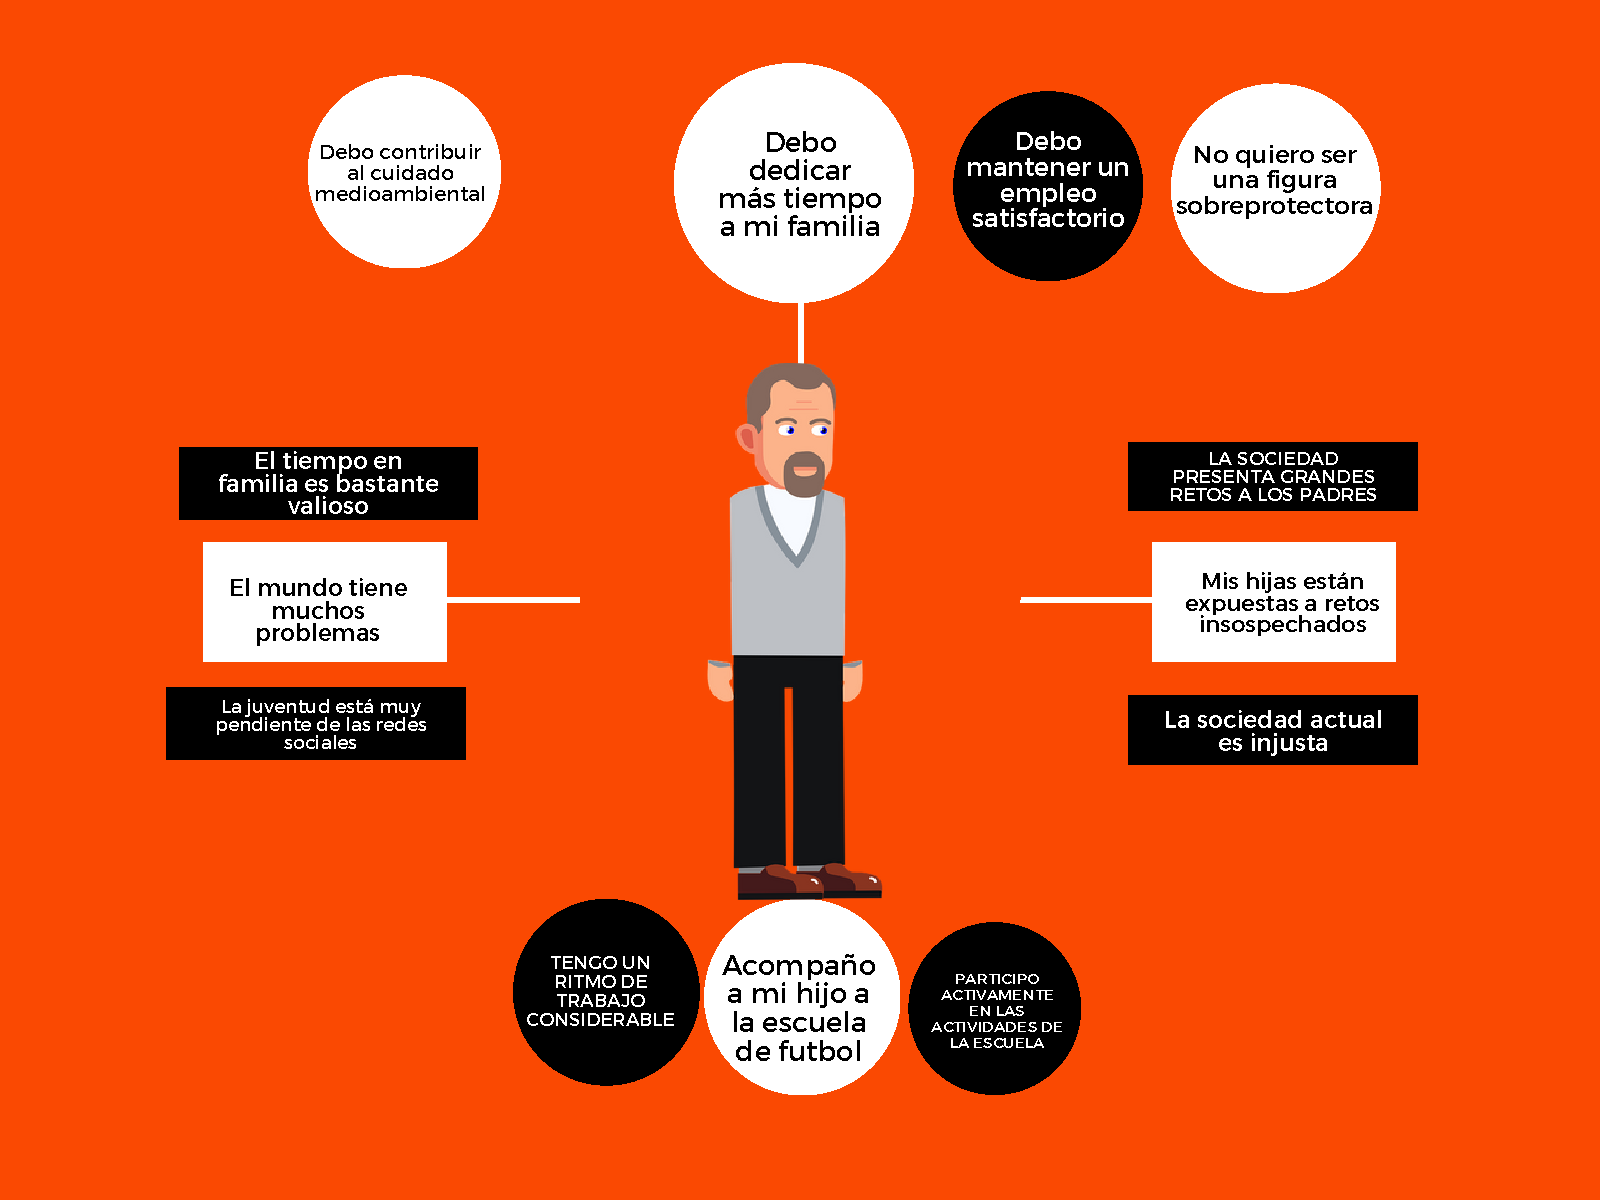
\includepdf[pages=-,landscape=True]{assets/build/mapa_de_empatia.pdf}

\newpage


\section{Jornadas del cliente}
\label{sec:orge9f5666}

\begin{figure}[htbp]
\centering
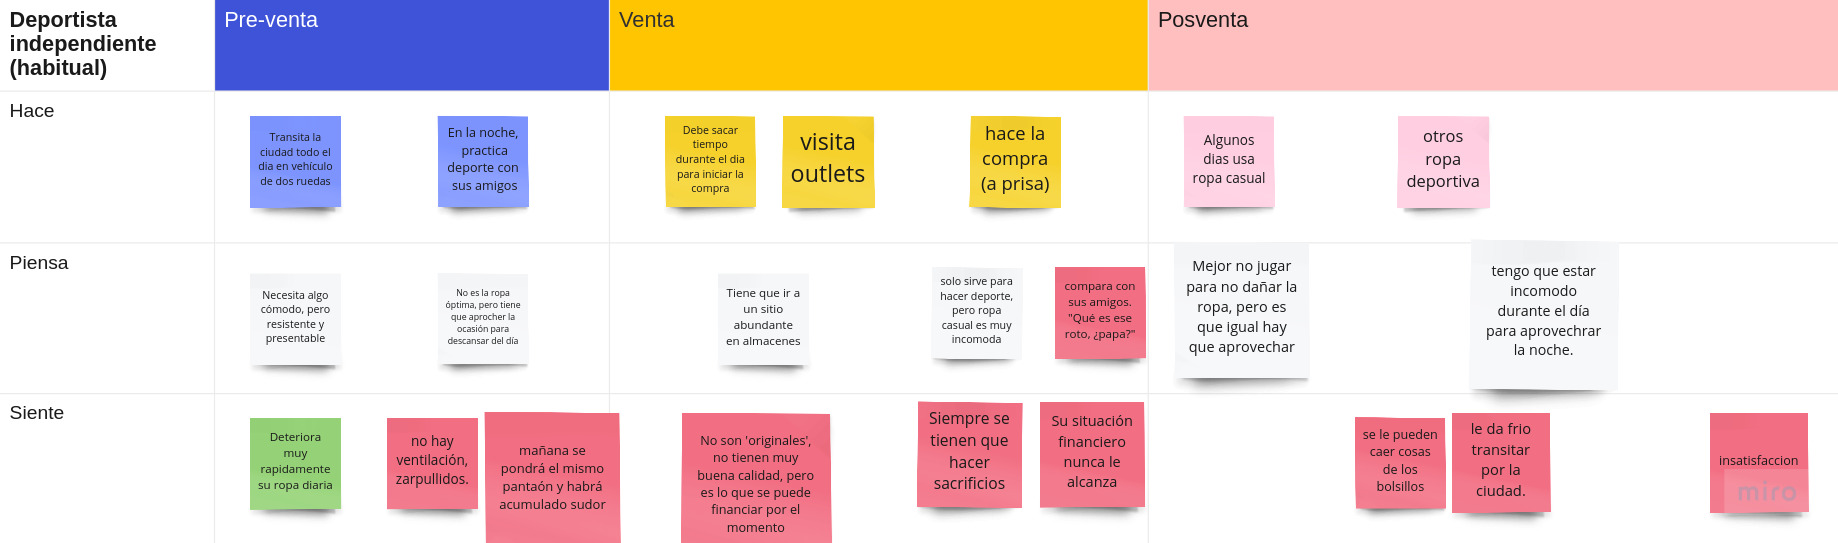
\includegraphics[width=.9\linewidth]{./entrega_jornadas/deportista_independiente_habitual.jpg}
\caption{Jornada 1}
\end{figure}
\begin{figure}[htbp]
\centering
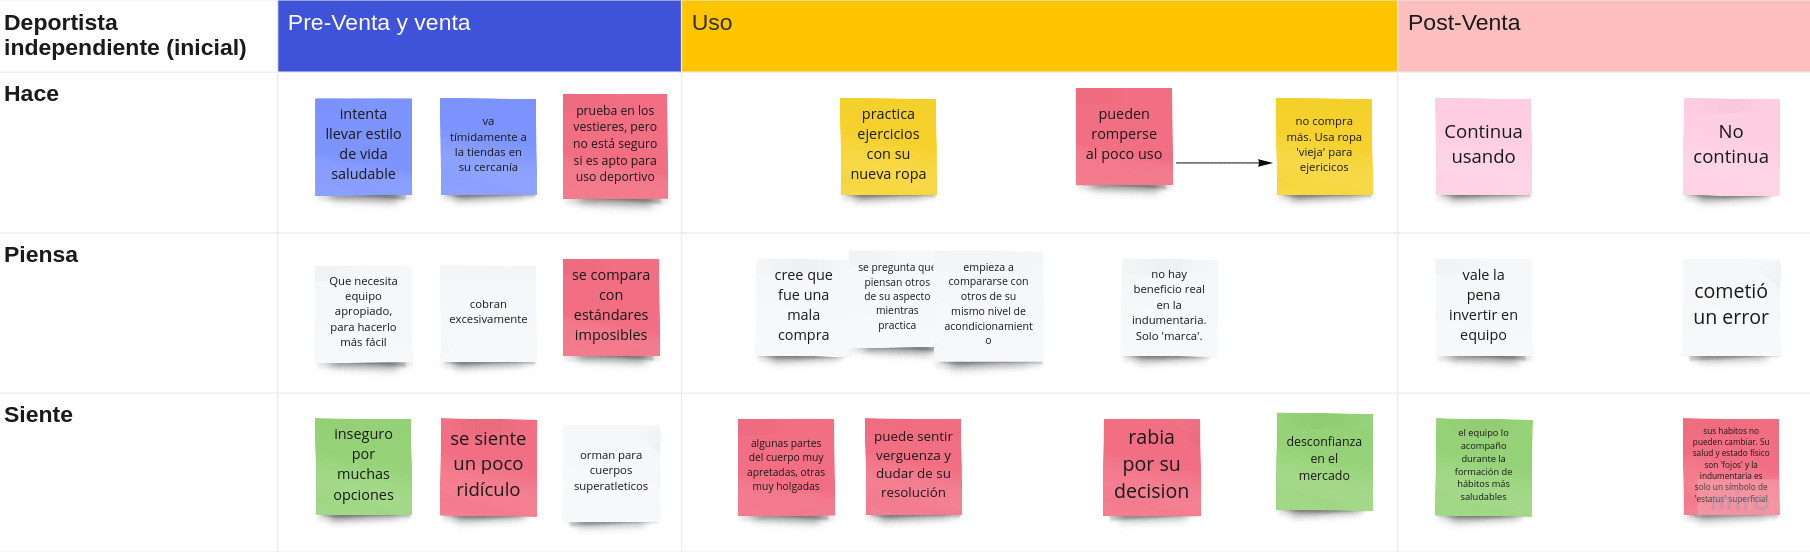
\includegraphics[width=.9\linewidth]{./entrega_jornadas/deportista_independiente_inicial.jpg}
\caption{Jornada 2}
\end{figure}
\begin{figure}[htbp]
\centering
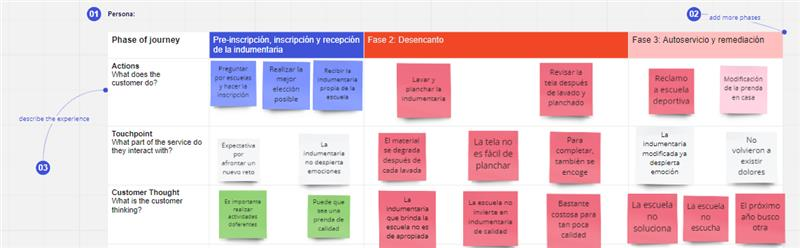
\includegraphics[width=.9\linewidth]{./entrega_jornadas/padre_de_familia.jpg}
\caption{Jornada 3}
\end{figure}


\newpage
\section{Ideación}
\label{sec:org2b197e2}
\subsection{Deportista independiente}
\label{sec:orgdecd8a1}
\begin{figure}[H]
\centering
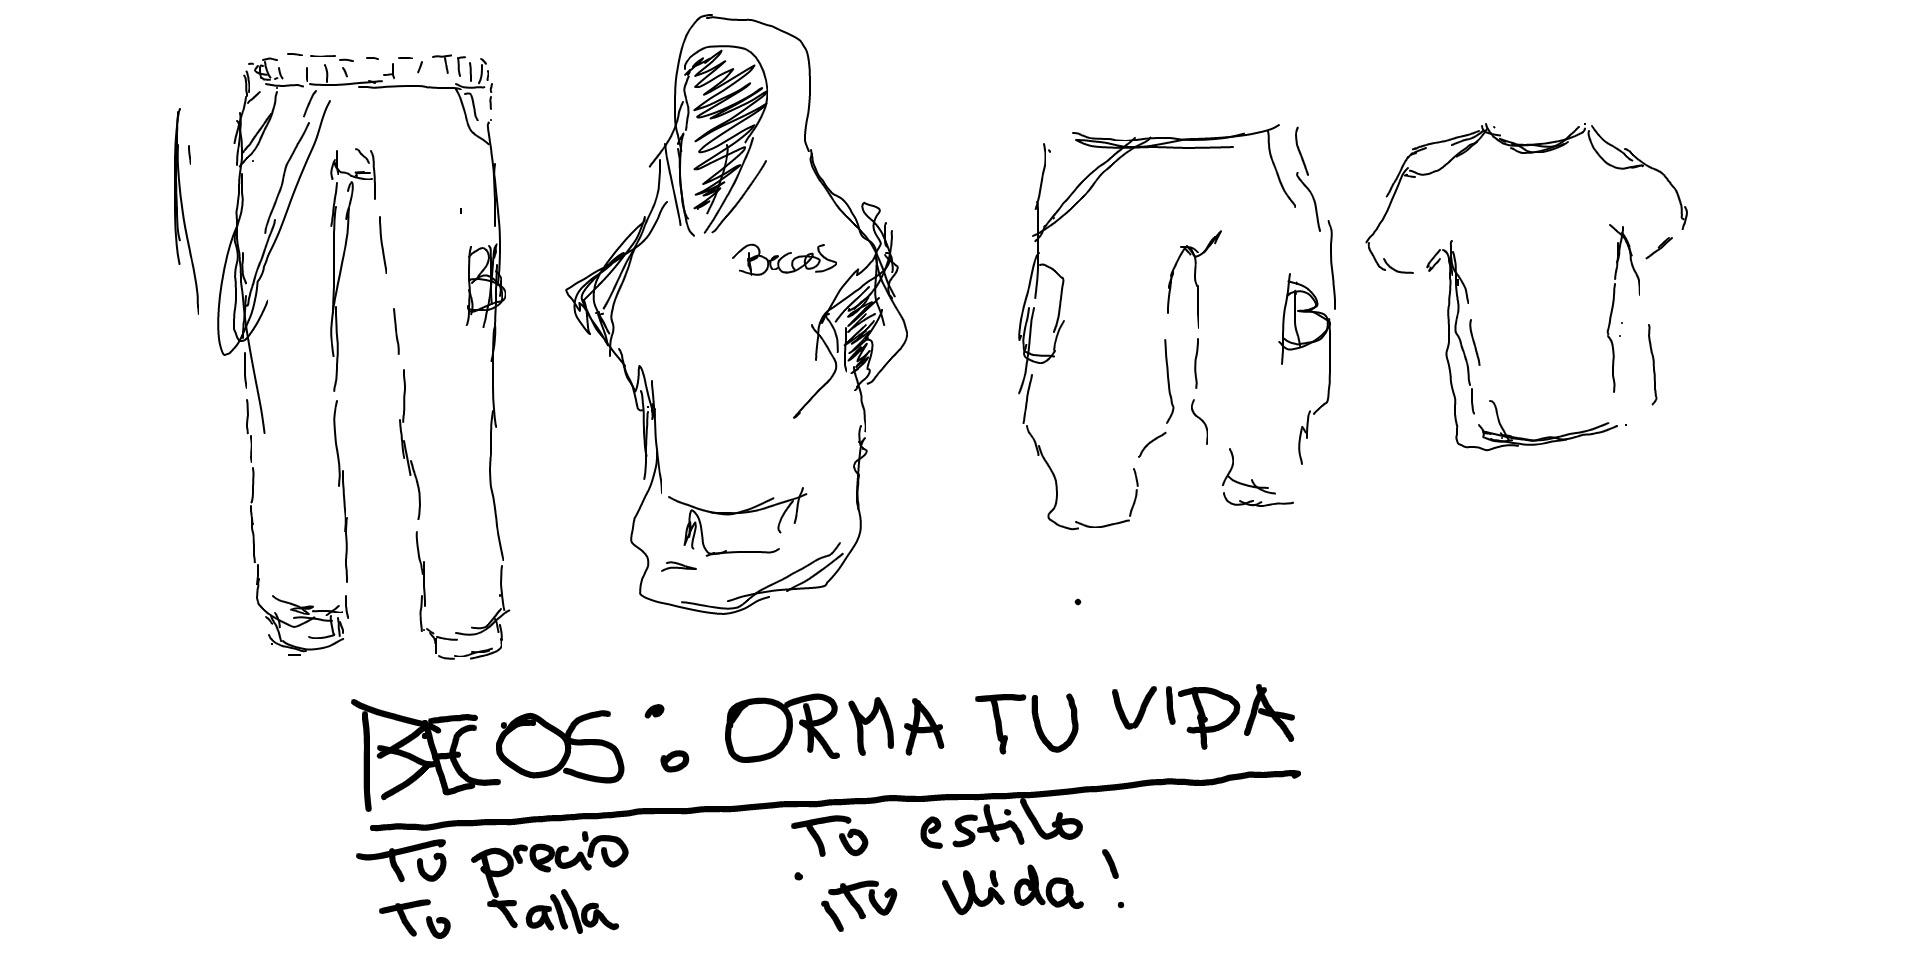
\includegraphics[width=.9\linewidth]{./assets/build/ideacion_1.jpeg}
\caption{Ideacion \#1}
\end{figure}



\subsection{Deportista de escuela}
\label{sec:org514e8e9}

\begin{figure}[H]
\centering
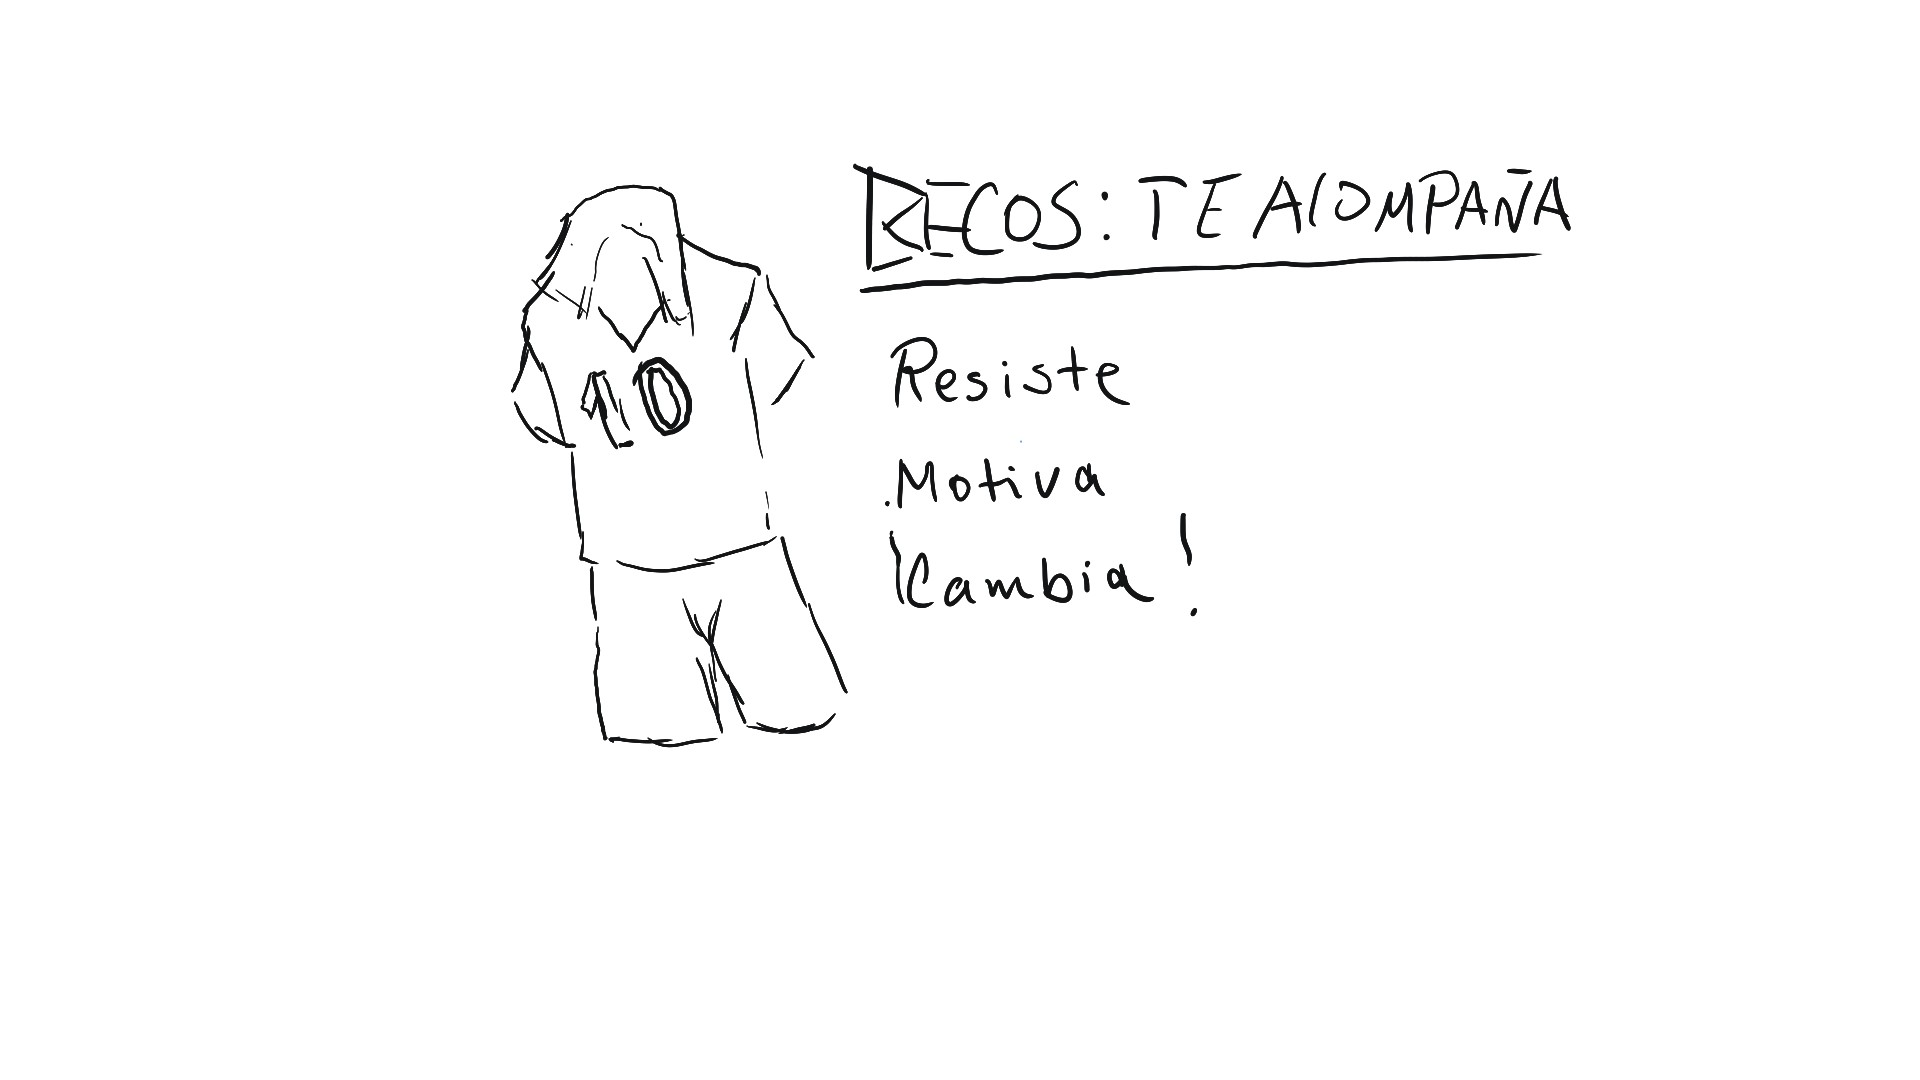
\includegraphics[width=.9\linewidth]{./assets/build/ideacion_2.jpg}
\caption{Ideacion \#2}
\end{figure}
\end{document}
